\ylDisplay{Maja} % Ülesande nimi
{Jaan Kalda} % Autor
{lõppvoor} % Voor
{2008} % Aasta
{G 4} % Ülesande nr.
{4} % Raskustase
{
% Teema: Varia
\ifStatement
Fotol kujutatud maja alumise korruse kõrgus (mõõdetuna esimese korruse akna alumisest servast teise korruse akna alumise servani) on 3 meetrit. Kui kõrgel veepinnast on maja (täpsemalt, tema vundamendi ülemine serv)?

\begin{center}
	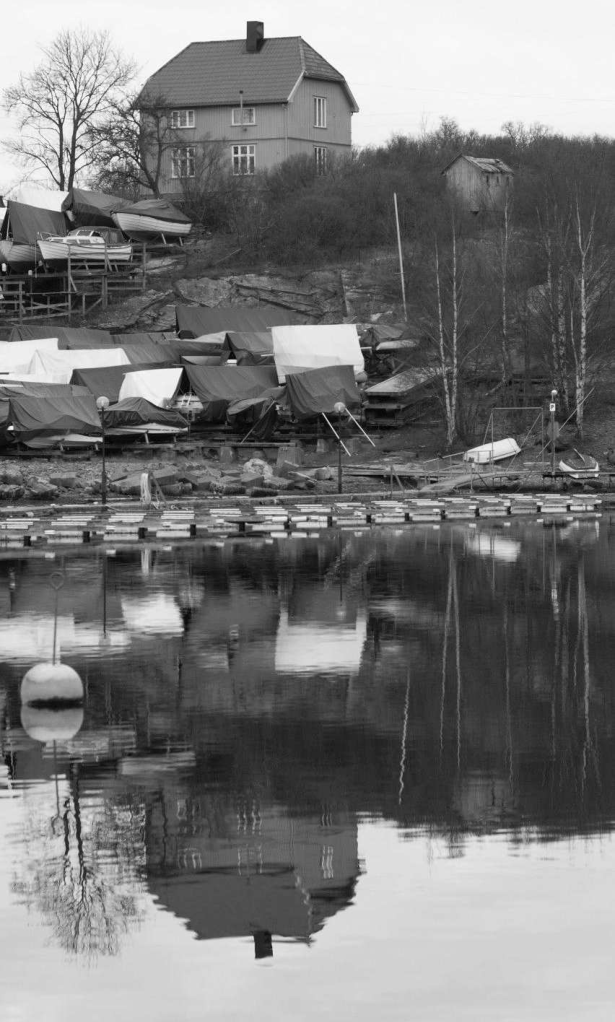
\includegraphics[height=\textheight]{2008-v3g-04-yl}
\end{center}
\fi


\ifHint
Maja teatud punkt ja tema peegelkujutis mere pinnalt paiknevad sümmeetriliselt mere tasandiga võrreldes. See võimaldab vee tasandi leidmist.
\fi


\ifSolution
Maja teatud punkt $P$ ja tema peegelkujutis mere pinnalt $P'$ paiknevad sümmeetriliselt mere tasandiga. Vaatleme mõttelist sirget $PP'$. Tema lõikepunkt merega $O$ paikneb mõlemast otsast võrdsel kaugusel ning tänu sellele saame me jooniselt punkti $O$ kergelt määrata kui lõigu $PP'$ keskpunkti. Maja kõrgus merepinnalt vastab vundamendi kaugusele punktist $O$, vt joonist. Mõõtes jooniselt akende vahekauguse $|AB| = \SI{9,5}{mm}$ ja $|OQ| = \SI{58,5}{mm}$ saame
\[
H = \SI{3}{m} \cdot \frac{|OQ|}{|AB|} = \SI{18,5}{m}.
\]

\begin{center}
	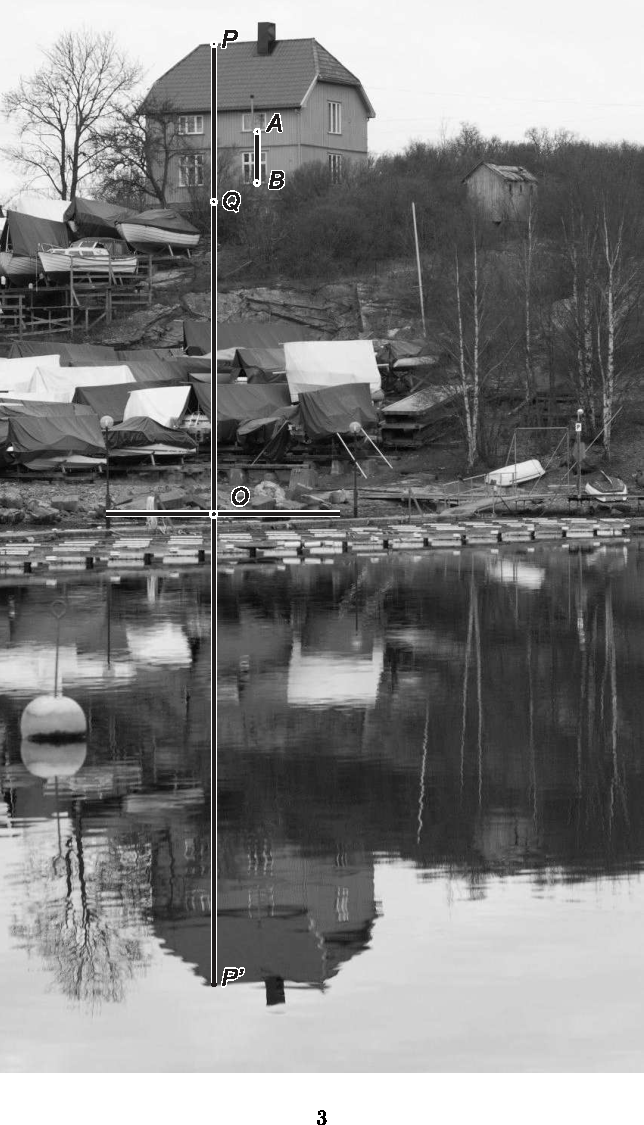
\includegraphics[height=\textheight]{2008-v3g-04-lah}
\end{center}
\fi
}